%LTeX: language=de-DE
\chapter{Gateway}
Das Gateway lässt die Applikation nach außen hin auf einen einzigen Port laufen. In Wirklichkeit laufen aber mehrere HTTP-Server, wie Frontend, Backend, Broker, zur selben Zeit auf verschiedenen Ports. Das Gateway startet auf Port 3000 und verteilt dann die Anfragen auf die verschiedenen Ports der anderen HTTP-Server.
Die ''main.ts'' des Gateways ist im Projektverzeichnis unter ''packages/gateway/src'' zu finden.
Der dazugehörige Codeausschnitt [siehe Abb. \ref{fig: gateway} auf S.~\pageref{fig: gateway}] zeigt wie das Gateway implementiert ist. 

\begin{figure}[h]
    \centering
    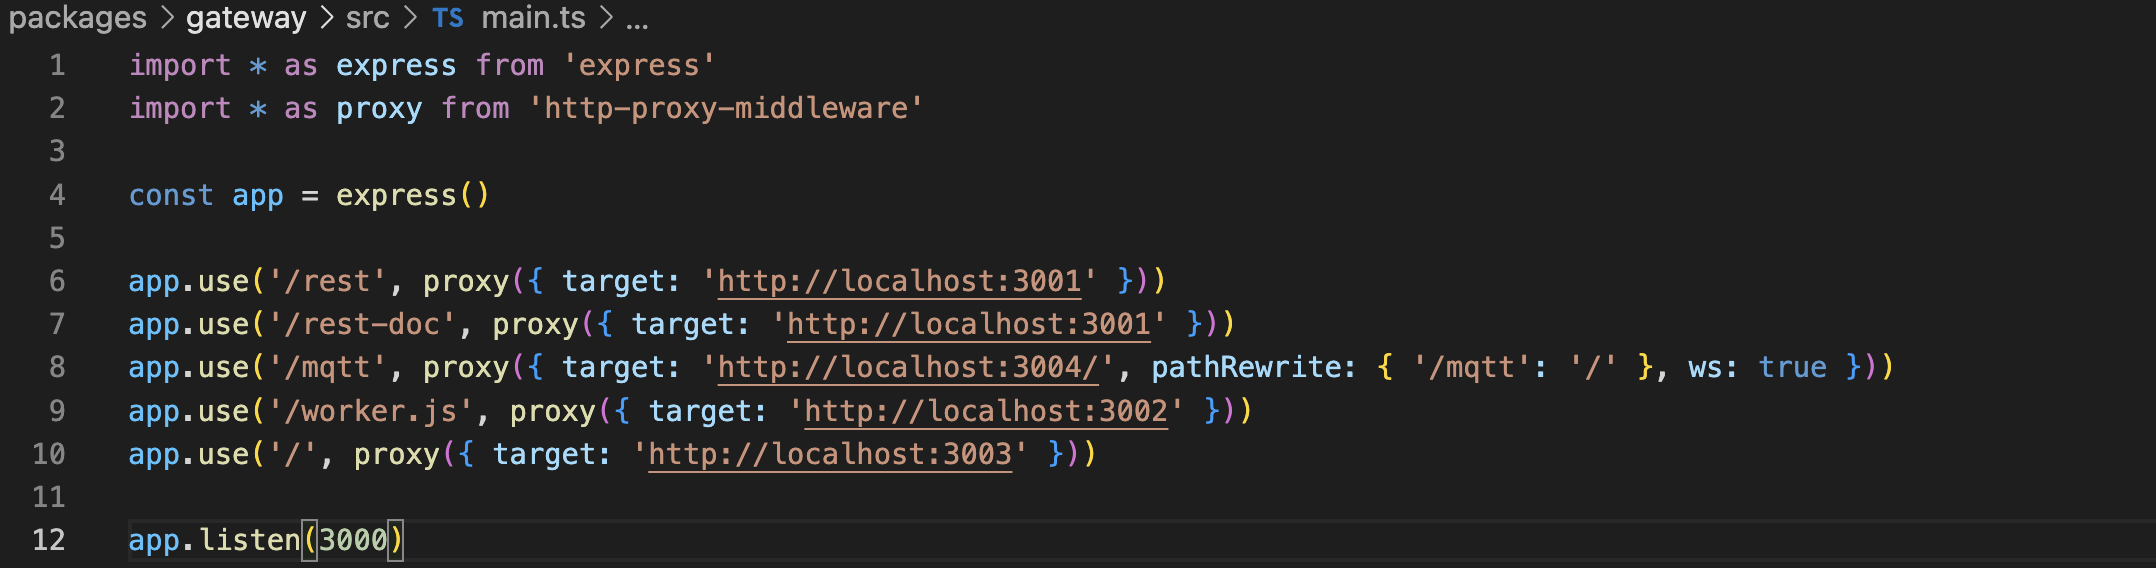
\includegraphics[width=1\textwidth]{gateway.png}
    \caption{Gateway}
    \label{fig: gateway}
\end{figure}